\PassOptionsToPackage{estonian,french,english}{babel} % example: to add additional languages
                                                      % last (english) is used by default
                                                      % temporary language switch is done by
                                                      % \begin{otherlanguage}{estonian}
\documentclass{TTUPhD}
%%%%%%%%%%%%%%%%%%%%%%%%%%%%%%%%%%%%%%%%%%%%%%%%%%%%%
%%%%%               Compiling                %%%%%%%%
%%%%%%%%%%%%%%%%%%%%%%%%%%%%%%%%%%%%%%%%%%%%%%%%%%%%%
% compile with:
%%%%%%%%%%%%%%%%%%%%%%%%%%%%%%%%%%%%%%%%%%%%%%%%%%%%%
% pdflatex thesis.tex
% bibtex thesis
% pdflatex thesis.tex
% pdflatex thesis.tex
%%%%%%%%%%%%%%%%%%%%%%%%%%%%%%%%%%%%%%%%%%%%%%%%%%%%%
% Note:
% because bibtex is used in 3 places (list of publ.,
% references section and publications appendix), then
% LaTeX warns about multiply defined BibTeX labels.
% This is normal.
%%%%%%%%%%%%%%%%%%%%%%%%%%%%%%%%%%%%%%%%%%%%%%%%%%%%%

%%%%%%%%%%%%%%%%%%%%%%%%%%%%%%%%%%%%%%%%%%%%%%%%%%%%%
%%%%% These can be used for revision process %%%%%%%%
%%%%%%%%%%%%%%%%%%%%%%%%%%%%%%%%%%%%%%%%%%%%%%%%%%%%%
%\usepackage{soul} % highlight text with \hl{highlighted text} 
%\usepackage{ulem} % strikethrough with \sout{stricken out text}
\usepackage{mathtools}
\usepackage{physics}
\usepackage{graphicx}
%\usepackage{setspace} %%% enable the
%\doublespacing        %%% double spacing 
%%%%%%%%%%%%%%%%%%%%%%%%%%%%%%%%%%%%%%%%%%%%%%%%%%%%%


\setlength{\parindent}{2em}
\setlength{\parskip}{1em}

%%%%%%%%%%%%%%%%%%%%%%%%%%%%%%%%%%%%%%%%%%%%%%%%%%%%%%%%%%%%%%%%%%%%%%%%%%%%%%%%%%%%%%%%%%%%%%
%%%%%%%%%%%%%%% user-defined variables used in several places of this document %%%%%%%%%%%%%%%
%%%%%%%%%%%%%%%%%%%%%%%%%%%%%%%%%%%%%%%%%%%%%%%%%%%%%%%%%%%%%%%%%%%%%%%%%%%%%%%%%%%%%%%%%%%%%%
% main information
\newcommand{\AuthorName}{Sammy Al Hashemi} % Author's name
\newcommand{\StudentNumber}{1001548337} % Author's name
\newcommand{\ThesisTitleENG}{Investigation into the scalability of Grover's Algorithm} % Title of thesis in English
\newcommand{\Year}{2019}
\newcommand{\ThesisTitleEST}{Doktorit\"o\"o pealkiri} % Title of thesis in Estonian
%%%%%%%%%%%%%%%%%%%%%%%%%%%%%%%%%%%%%%%%%%%%%%%%%%%%%%%%%%%%%%%%%%%%%%%%%%%%%%%%%%%%
%%%%%%%%%%%%%%%%%%%%%%%%%%%%%%%%%%%%%%%%%%%%%%%%%%%%%%%%%%%%%%%%%%%%%%%%%%%%%%%%%%%%
% list of bibliography resource files
\newcommand{\BibResources}{references} % list here the bibliography resources used in the work
                                          % that means .bib files with absolute or relative paths,
                                          % separated by a comma (no space). Here the file
                                          % './references.bib' is used
                                          
%%%%%%%%%%%%%%%%%%%%%%%%%%%%%%%%%%%%%%%%%%%%%%%%%%%%%%%%%%%%%%%%%%%%%%%%%%%%%%%%%%%%%%%%%%%%%%
%%%%%%%%%             end of common variables (used in several places)                 %%%%%%%
%%%%%%%%%%%%%%%%%%%%%%%%%%%%%%%%%%%%%%%%%%%%%%%%%%%%%%%%%%%%%%%%%%%%%%%%%%%%%%%%%%%%%%%%%%%%%%




\begin{document}
\begin{centering}

%First title  page, English. Should require no manual modification
{\large
 University of Toronto\\
}
\vspace{5.5CM}
{\huge
\bf{
\ThesisTitleENG \\
}
}
\vspace{4.2cm}
{\fontsize{16}{19.2} \selectfont \MakeUppercase{\AuthorName}} \\
{\fontsize{16}{19.2} \selectfont \MakeUppercase{\StudentNumber}} \\
\vspace{7cm}%{7.9cm} %PRESS\\
\end{centering}
\thispagestyle{empty}
%%%%%%%%%%%%%%%%%%%%%%%%%%%%%%%%%
\newpage 



% inverse side of first title page: data (MODIFY!)
\thispagestyle{empty} 
{\noindent 
University of Toronto \\                    % MODIFY!
Department of Engineering Science \\                 % MODIFY!
 }
\noindent
\vspace{-3mm}

\begin{tabbing}
\textbf{Supervisor:} \quad \quad\= Glen Gulak,\\ % MODIFY!
\>{\small Department of Electrical and Computer Engineering} \\ % institute goes here
\>{\small University of Toronto} \\ % uni. and country
\>{\small Toronto, Canada} \\ % uni. and country
\\
\end{tabbing}

\noindent
\textbf{Defence of the thesis:} April \Year, Toronto \\ % MODIFY!

\clearpage
\thispagestyle{empty}


% its inverse, empty
\thispagestyle{empty}
$ \quad $
\newpage


% if table of contents is too long, then use the 'spacing' commands: 
%\begin{spacing}{0.1}
\tableofcontents
%\end{spacing}



\section*{Symbols (if needed)} % here section automatically starts at odd-numbered fresh page
\addcontentsline{toc}{section}{Symbols} 
\begin{tabular}{p{2cm} p{8cm}}
... & ... \\
... & ... \\
... & ... \\
... & ... \\
\end{tabular}

\clearpage
\listoffigures
\addcontentsline{toc}{section}{List of Figures} 

\clearpage
\listoftables
\addcontentsline{toc}{section}{List of Tables} 
(if needed)


\section{Introduction}
\subsection{Background Information}
\addcontentsline{toc}{section}{Introduction}  % adds unnumbered section to the table of contents

 The idea of a quantum computers was first proposed by Richard Feynman in 1982, as a possible solution to solve programs that could not be solved in polynomial time on a classical computer [1]. This sentiment has inspired a movement in favour of development of large-scaled quantum computers and has recently risen to the forefront in many tech giants such as Google, IBM, Microsoft, and Alibaba [2]. Recent preliminary results on smaller-scale quantum processors with up to 20 qubits have demonstrated the capability of the hardware to be programmed and controlled. The biggest challenge lies ahead in efforts to reduce the hardware limitations currently available. This is an incredible challenge going forward as it requires physical qubits well isolated from the environment and capable of being addressed and coupled to more than one extra qubit [3]. However, there has been massive progress recently, as the largest tech giants compete to build the first commercially available quantum computer [2]. For example, Google recently announced Bristlecone, their new 72-qubit quantum processor while Rigetti announced their own 128-qubit chip [14]. Although Google is �cautiously optimistic�, this is very exciting as it has been proposed that quantum devices with more than ~50 qubits are expected to perform certain algorithms better than classical computers, thus achieving quantum supremacy [4][5].
 
 The implications of the emergence of quantum computing are very great, particularly when considering the strength of modern data security for major companies, banks and blockchains [7]. Two quantum algorithms that are of utmost importance in this context are Shor�s (prime factorization) and Grover�s (unstructured database query) algorithms [9][13]. Classical computers do not possess the power to overcome the computational effort required to break modern encryption methods, which in the case of RSA key encryption, require the prime factorization of very large numbers, and lattice-based encryption schemes often require solving a variant of the shortest vector problem (SVP). The emergence of Shor�s algorithm is currently of main concern due to its threat on the most popular encryption algorithms, such as RSA encryption. Grover�s algorithm presents further threats to encryption algorithms proposed in response to Shor�s, due to its ability to solve cryptographic hashing and ease the complexity in solving SVP and AES encryption [6][7][8].

\subsection{Objective of this paper}
While Grover�s algorithm is a clearly defined problem, and early versions do exist, there is room to invest in its practicality and scalability, as quantum computers continue to evolve past their current limitations. Grover�s algorithm assumes the existence of a �magical� black-box oracle function that identifies when any �winning� value exists, while searching in an unstructured database [9]. Early implementations use quantum circuits with oracles precompiled for predefined values [9][10][11][12]. The objective of this research, is to develop a practical oracle function for use in Grover�s algorithm in any scalable system and create benchmark tests to estimate and measure the runtime on actual hardware. To do so, and initial step of extensive literature review, and public consultation of forums specific to the quantum computing community, is considered. To test and validate what has been done, small-scale circuits will be built for execution on currently available simulation engines such as Rigetti Forest and IBM Quantum Experience. The hardware will be accessed through various platforms for quantum algorithm development. These platforms include IBM Quantum Experience�s 16 qubit processor available for public use over the cloud using their python SDK, as well as Rigetti's Forest SDK implementing their Pyquil library. For each test attempted, the complexity and accuracy of each presented oracle will be judged. Once confident that a valid practical implementation of an oracle has been demonstrated, the remainder of the paper will deal with introducing parameterization for scalability of the algorithm.

In the sections to follow, the fundamentals of quantum mechanics necessary to understand quantum computation, the basis of quantum computation, the current state of quantum hardware, and a detailed explanation of Grover's algorithm will follow. Specifically, in our discussion of Grover's algorithm, the abstract definitions of the main components will first be discussed, then several implementations of those components will be compared; particularly for the overtly abstract Grover's oracle function.

\section{Quantum Background}
In essence, computers are all about the ability to store and process information, and the ability to operate on the information given to them. Classical computers encode information in registers, or in a more abstract sense, bits. These bits can take a value of $0$ or $1$, with more complex pieces of information requiring more bits to be fully encoded. These bits are determinate, as in one can know what there value concretely, and can accurately predict its value after several operations. Quantum computing, as a whole, relies on the fundamental concepts of quantum mechanics to encode the information. It abstracts the concept of the bit found in classical computers to a non-deterministic 'qubit', which will be covered later. Thus, in order to grasp the nature of quantum computing, a solid background in quantum mechanics is fundamental.

\subsection{The Quantum State and Quantum Operations}
In many ways,the goal of physics is to be able to describe a system in question and to be able to predict the future of a system based on the current information known. For example, a classical system of a ball rolling may be described by the ball's position, its velocity, and its acceleration. Knowing this, the balls future position, say after $t$ seconds, can be predicted. The quantum state is an abstraction of this. In quantum mechanics, the quantum state is also referred to as the \textit{wavefunction}. The wavefunction contains all information regarding a quantum system. The difference between a classical state and a quantum state, as previously highlighted, is the deterministic nature of the classical state: as opposed to a quantum system, one can accurately predict the future state of a classical system. Quantum systems operate in \textit{probability land}; that is, having known the previous state of a system, you can only predict the future state of a system with a \textit{degree of confidence}. One only truly knows the future state once it has been measured. This is referred to as \textit{collapsing the wavefunction}. In this instance, the wavefunction has collapsed onto whatever future state was measured. 

A quantum operation is an operation that transforms one wavefunction into another. In the classical example of a ball rolling, an example of an operation would be to push the ball with force, $F$. As before, using this information that the ball has been pushed in addition to the previous information of the ball before the push lets the ball's future state be deterministically predicted. In the quantum analogue, the quantum operation transforms the state into a new state, but this new state will be unknown until it has been measured. Quantum operations can have many properties; for example, those that are \textit{unitary} are referred to as being \textit{reversible}. That is, if acted twice on a wavefunction, they return the exact same wavefunction.


\subsection{Common Notation}
A wavefunction in nature is an abstract concept. To represent it, and more importantly to represent any operations on a wavefunction, a strict notation should be followed. To do this, we follow \textit{Dirac Notation}. In Dirac Notation, the wavefunction is represented by \[\ket{\Psi}\]

which is called a ket. Since kets can be represented as column vectors in a particular basis, which will be discussed shortly, one can enact linear algebra operations on it. Namely, the \textit{Hermitian Conjugate} is called the bra: \[\ket{\Psi}^\dag = \bra{\Psi}\] The \textit{inner product} of two wavefunctions is abstractly defined by a bra being projected onto a ket: \[\braket{\Psi 1}{\Psi 2}\] For a quantum operator, $A$, the expectation value of $A$ is:
\[\left\langle \Psi \middle| A \middle| \Psi \right\rangle\]


\subsection{Quantum Basis}
With the wavefunction being such an abstract concept, it's hard to get any true encoding of a quantum state. To do so, one can project the wavefunction onto various bases. For example, the wavefunction can be projected onto the \textit{position basis}, which is an infinitely large basis, as there are an infinite amount of possible positions to be occupied: $\Psi(x) = \braket{x}{\Psi}$. The same can be done for another basis, the \textit{momentum basis}: $\Psi(p) = \braket{p}{\Psi}$. Just like the position basis, the momentum basis is also of infinite size as there are an infinite amount of momentum values to take. These two are called \textit{continuous bases} due to their infinite number of possible states to be taken. As opposed to continuous bases, \textit{discrete bases} have a finite amount of possible states to be taken, and thus are of finite dimension. One such example of a discrete basis is the magnetic spin states: $(\ket{0}, \ket{1})$. A wavefunction projected onto this basis is often referred to as a \textit{spinor}. Just like in the continuous case, a wavefunction can be represented in this basis by being projected onto the basis states: $\braket{0}{\Psi}$ and $\braket{1}{\Psi}$. The important realization of the basis representation comes about in the next section where when measuring a wavefunction, there is a probability of being measured in each basis state. In this case of the spinor, there is a probability of being in the $\ket{0}$ state and a probability of being in the $\ket{1}$ state.

\subsection{Quantum Superposition and Vector Representation}
In a particular basis, a wavefunction can be represented by a superposition of the basis states. For example, in the discrete magnetic spin basis, a wavefunction may be represented by: \[\ket{\Psi} \rightarrow \alpha \ket{0}  + \beta \ket{1}\]
Here, $\alpha = \braket{0}{\Psi}; \beta = \braket{1}{\Psi}$. The values $(\alpha, \beta)$ are the complex coefficients on expansion of the wavefunction in the basis, or "what proportion of the wavefunction is projected onto each basis". It can thus be written as: \[\ket{\Psi} \rightarrow \begin{bmatrix} \alpha \\ 0  \end{bmatrix} + \begin{bmatrix} 0 \\ \beta \end{bmatrix}\]
\[\ket{0} = \begin{bmatrix} 1 \\ 0  \end{bmatrix}; \ket{1} = \begin{bmatrix} 0 \\ 1  \end{bmatrix}\]

Note that the bra representations of the basis states are instead row vectors:
\[\ket{0} = \begin{bmatrix} 1 & 0  \end{bmatrix}; \ket{1} = \begin{bmatrix} 0 & 1  \end{bmatrix}\] The \textit{representation} of a quantum operator, $A$, in a basis, for example in the same $2-dimensional$ basis we have been working in is as follows:
\[A \rightarrow \begin{bmatrix} \left\langle 0 \middle| A \middle| 0 \right\rangle & \left\langle 0 \middle| A \middle| 1 \right\rangle \\ \left\langle 1 \middle| A \middle| 0 \right\rangle & \left\langle 1 \middle| A \middle| 1 \right\rangl \end{bmatrix}\]

If one computes the inner product of the wavefunction with itself: \[\braket{\Psi}{\Psi} = |\alpha|^2 + |\beta^2|\] 
it is noteworthy that for a normalized wavefunction: $\ket{\Psi}$, $|\alpha|^2 + |\beta|^2 = 1$. Therefore, $(|\alpha|^2, |\beta|^2)$ are the respective probabilities of the wavefunction collapsing on the state associated with it. For a wavefunction projected onto a discrete $n-dimensional$ basis, the probability of the wavefunction being found in the $i^{th}$ state, $\ket{i}$, is 
\[p_i = |\braket{i}{\Psi}|^2\]


\subsection{Hilbert Space \& Bloch Sphere}
The \textit{Hilbert Space} is defined as a vector space where all wavefunction of a system exist; that is all possible states that are available. The basis states that the wavefunction has projected on are the basis vectors that span this entire space. For a $2-dimensional$ basis, an equivalent description of the Hilbert Space is called called the \textit{Bloch Sphere} (it can be generalized to more dimensions, however). The Bloch Sphere provides a nice visualization for quantum states in spherical coordinates [15]. For example, staying with the $(\ket{0}, \ket{1})$ basis, the arbitrary wavefunction can be instead written as:
\[\ket{\Psi} = cos(\theta / 2) \ket{0}  + e^{i\phi}sin(\theta / 2) \ket{1}\]
\[|cos(\theta / 2)|^2 + |e^{i\phi}sin(\theta / 2)|^2 = 1\]
\[0 \leq \theta \leq \pi \]
\[0 \leq \phi \leq 2\pi\] 
With this parameterization, any point on the surface of the Bloch Sphere can be covered by a quantum state of the system in question. \textbf{INSERT PICTURE OF BLOCH SPHERE HERE}

With the Bloch Sphere representation in mind, some important states that concern us in regards to quantum computing are the states along the $+z$ axis, $\ket{0}$ and the $-z$ axis, $\ket{1}$. Several other important states are the normal superpositions of $(\ket{0}, \ket{1})$. They are:
\[\ket{+} = \frac{\ket{0} + \ket{1}}{\sqrt{2}} \; \ket{-} = \frac{\ket{0} - \ket{1}}{\sqrt{2}}\]

\subsection{Coherence}
In quantum mechanics, the states of a system are said to be \textit{coherent} if they maintain constant phase relations. In the Bloch Sphere representation presented above, this means that the $\ket{+}$ and $\ket{-}$ states are always along the $+z$ and $-z$ axes. A system's coherence is fundamental is fundamental in quantum mechanics and is necessary for a perfectly functional quantum computer. In cases where a system isn't completely isolated, and thus may interact with its environment, these states may lose their constant phase relations. This process is called decoherence and it is very important that a quantum computer maintain \textit{extremely} low decoherence or else suffer the possibility of loss of information.

There are two main decoherence processes, one being \textit{energy relaxation}, the other being \textit{dephasing}. Energy relaxation is the result of an excited state losing energy to its environment [16]. For example, this could be the $\ket{+}$ state decaying to the $\ket{0}$ state. It is important for the time constant, $T_1$ of this process to be very large for a quantum computer. On the other hand, dephasing leads to loss of coherence as a result of perturbations of the quantum system over time [16]. Like energy relaxation, it is important that the time constant for this process, $T_2$, also be very large. Much progress has been made in the past two decades in improving the coherence of quantum computers. As an example, consider this plot provided by \textit{IBM} displaying the improved coherent times of their quantum computers over time: \textbf{INSERT IBM COHERENT PICTURE HERE}
\begin{figure}[h!]
    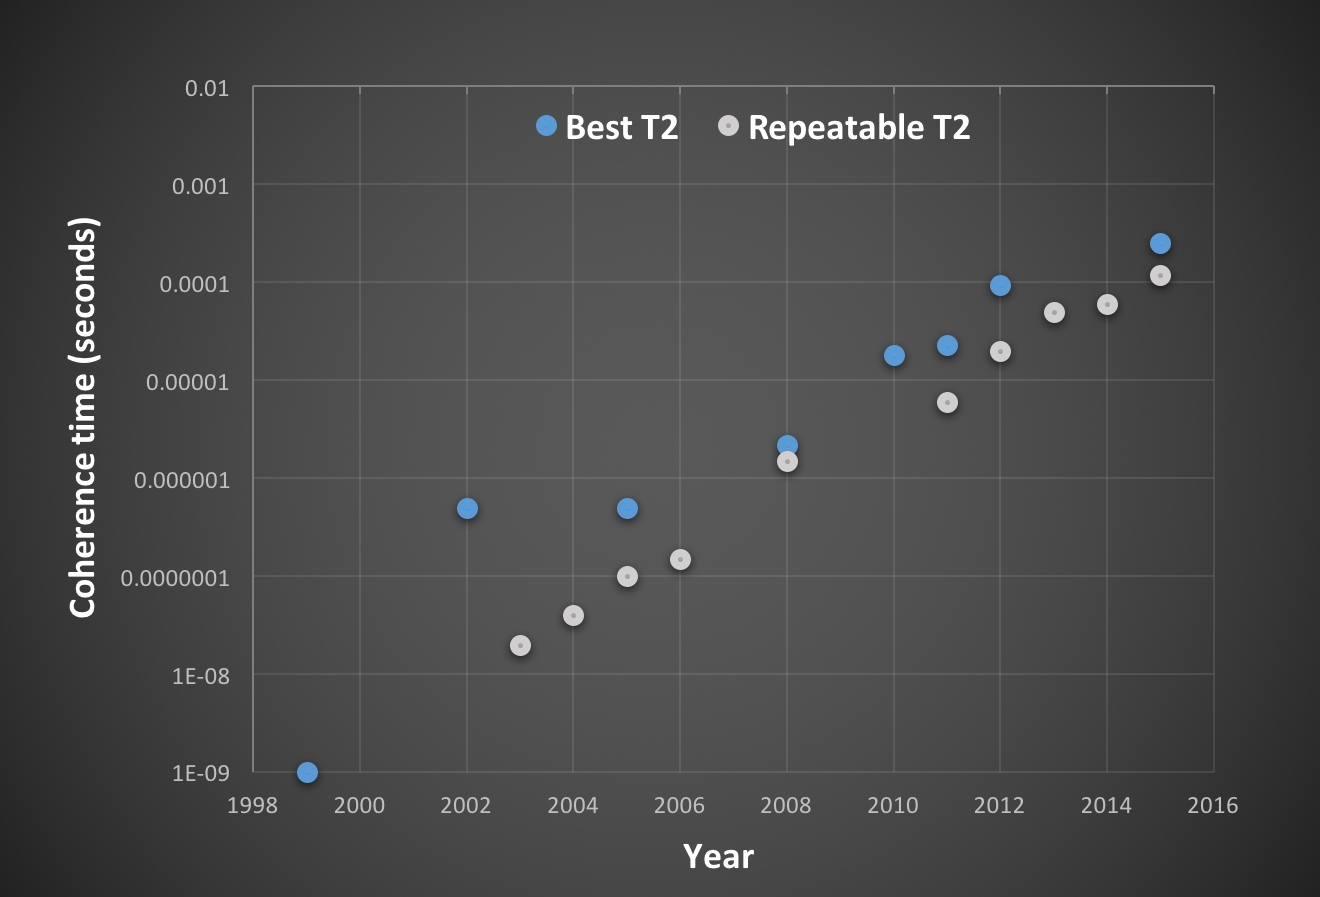
\includegraphics[width=\textwidth]{IBMQ_coherence.png}
    \caption{Decoherence time constants of IBMQ hardware [16]}
    \label{fig1.}
\end{figure}


\section{Quantum Computation}
Quantum computation has exponentially grown in interest over the last few years, partly due to threats in cybersecurity, partly due to the proven advancements and benefits in scientific research it could impact, and partly due to the desire to achieve quantum supremacy [17]. This sentiment has inspired a movement in favour of development of large-scaled quantum computers and has recently risen to the forefront in many tech giants such as Google, IBM, Microsoft, and Alibaba [2]. As an example, Google recently announced Bristlecone, their new 72-qubit quantum processor while Rigetti announced their own 128-qubit chip [14]. Google is �cautiously optimistic�, but this is very exciting as it has been proposed that quantum devices with more than ~50 qubits are expected to perform certain algorithms better than classical computers, thus achieving quantum supremacy [4][5]. In this section several models of quantum computing will be introduced and compared, the most common of these models being the \textit{qubit model} and the \textit{continuous variable model}.

\subsection{Models of Quantum Computation}
As opposed to classical computers, which encode information a series of $0/1$ strings in bits, which are deterministic in nature, quantum computers try to take advantage of the probabilistic nature of quantum states to encode information in abstractions of bits that depend on the kind of model implemented. In the qubit model, the \textit{qubits} is used to encode information while in the continuous variable (CV) model, the \textit{qunat} is used to encode information.

\subsection{Qubit Model}

\subsubsection{The Quantum Bit}
The qubit model of quantum computing encodes information in a qubit. A qubit is a quantum state projected on a $2-dimensional$ state space. This means, just like the wavefunction expanded in terms of the magnetic spin states $(\bra{0}, \bra{1})$, there are only two states it can collapse to, when measured. In fact, the most common mathematical representation of a qubit is in the magnetic spin basis [19]. In any other case it can be in the arbitrary state:
\[\ket{\Psi} = \alpha\ket{0} + \beta\ket{1}\]
One may ask: how come it can only collapse onto one of two states when the general state is written in terms of two different states? This is because when measuring, the quantum realm is exited and in the classical realm, something cannot be in two different states at once [15]. This is due to the \textit{Uncertainty Principle} [15].


\subsection{Quantum Operations in the Qubit Model}
In classical computer, logical operations on bits mutate their \textit{value}, sometimes depending on the values of other bits. In the qubit model of quantum computing, the \textit{probabilities} of a qubit are modified, in effect altering the linear combination of the $\ket{0}$ and $\ket{1}$ states. However, there are certain restrictions put on a quantum operator. These restrictions follow straight from fundamental laws of physics [18]. Specifically, what needs to be followed is according to the \textit{Second Law of Thermodynamics} which states that the total entropy of a closed system must never decrease. What this implies is that a quantum operator must be \textit{reversible}. If the same quantum operator is applied to a wavefunction twice and it spits out a new wavefunction, this means that some information regarding the initial state was lost. As discussed previously, a reversible quantum operator preserves all information about the initial state. An example of a reversible operator from classical computation is the NOT gate. The other requirement surrounding quantum operators is that they must be \textit{unitary} to preserve the probability amplitude of the states. That is, after the operator has been applied, the condition 
\[|\alpha|^2 + |\beta|^2 = 1\]
must still apply. To see a proof that all unitary operators that are unitary preserve the probability amplitude, consult \textbf{Appendix A}. 

\subsubsection{Operations on Single Qubits}
The NOT gate actually belongs to a group of operators called the \textit{Pauli operators}. The Pauli operators are derived from the general spin operator that acts on spinors, $S$. To derive the NOT gate, or the $X$ gate, we can work in the $(\bra{0}, \bra{1})$ basis:
\[\begin{pmatrix} \begin{bmatrix} u_{00} & u_{01} \\ u_{10} & u_{11} \end{bmatrix}\begin{bmatrix} 1 \\ 0 \end{bmatrix} = \begin{bmatrix} 0 \\ 1 \end{bmatrix} \\ \\ \begin{bmatrix} u_{00} & u_{01} \\ u_{10} & u_{11} \end{bmatrix}\begin{bmatrix} 1 \\ 0 \end{bmatrix} = \begin{bmatrix} 0 \\ 1 \end{bmatrix} \end{pmatrix} \rightarrow X = \begin{bmatrix} 0 & 1 \\ 1 & 0 \end{bmatrix}\]
The other Pauli operators are as follows:
\[Y = \begin{bmatrix} 0 & -i \\ i & 0 \end{bmatrix} \; Z = \begin{bmatrix} 1 & 0 \\ 0 & -1 \end{bmatrix}\]
The Pauli operators $X, Y, Z$ perform rotations of $\pi$ radians around the $x, y, z$ axes respectively of the Bloch Sphere. One more idea to notice is the dimensionality of the matrices that operate on single qubits, such as the Pauli gates: they are of dimension $2$. As the number of qubits a gate operates on increases, the dimensionality of the operators increases as well.
Another very important unitary operator that acts on a single qubit is the Hadamard gate, $H$. This gate creates an equal superposition of both basis states $(\ket{0}, \ket{1})$. Namely:
\[H\ket{0} = \frac{\ket{0} + \ket{1}}{\sqrt{2}} =  \ket{+} \; H\ket{1} = \frac{\ket{0} - \ket{1}}{\sqrt{2}} = \ket{-}\]
Also note that (similarly for $\ket{1}$):
\[HH\ket{0} = \ket{0}\]
Other important single-quibt gates include the \textit{rotation gates} $R_x(\theta), R_y(\theta), R_z(\phi)$ which are parameterized gates that rotate the qubit around the $x, y, z$ axes of the Bloch sphere respectively, the S gate, which introduces a phase rotation of $\pi /2$, and the T gate, which introduces another phase rotation of $\frac{1 + i}{\sqrt{2}}$.

\subsubsection{Square root of quantum gates}
Classically, if one has a function $f(x)$ that maps $x$ to a new number, it is unusual to think of the existence of $\sqrt{f(x)}$. However, every quantum gate does have a defined square-root [20]. That is, consider the NOT gate, $X$, there does in fact exist a $\sqrt{X}$ such that:
\[\sqrt{X}\sqrt{X} = X\] 
As an example, the matrix representation of $\sqrt{X}$ will be derived. To do so, we shall look for the eigendecomposition of the $X$ gate [20]. The $X$ gate has eigenvalues and eigenvectors:
\[\lambda = \pm 1 \; v = \begin{bmatrix} 1 \\ \pm 1 \end{bmatrix}\]
The eigendecomposition is therefore: 
\[X = \lambda_1 v_1v_1^\dag + \lambda_2 v_2v_2^\dag\]
Eigendecompositions are nice because when operations are performed on a matrix, they usually just correspond to transforming the eigenvalues [20]:
\[\sqrt{X} = \sqrt{\lambda_1} v_1v_1^\dag + \sqrt{\lambda_2} v_2v_2^\dag\]
\[\therefore \sqrt{X} = \frac{1}{2} \begin{bmatrix} 1+i & 1-i \\ 1-i & 1+i \end{bmatrix}\]
One can easily verify that this matrix is unitary.

\subsubsection{Z-Y decomposition}



\subsubsection{Systems with multiple qubits}
For systems with more than one qubit, subtle complexities start to arise, namely entanglement. Entanglement is the phenomenon where the quantum state of one qubit cannot be described without information about the other qubits in the system. To describe the new entangled states of the system mathematically, a new set of basis states must be constructed. To do so, we construct them out of \textit{direct product} states of the single qubit states. That is, using the example of a two qubit system:
\[\ket{00} = \ket{0} \bigotimes \ket{0} = \begin{bmatrix} 1 \\ 0 \\ 0 \\ 0 \end{bmatrix} \; \ket{01} = \ket{0} \bigotimes \ket{1} = \begin{bmatrix} 0 \\ 1 \\ 0 \\ 0 \end{bmatrix} \: \ket{10} = \ket{1} \bigotimes \ket{1} = \begin{bmatrix} 0 \\ 0 \\ 1 \\ 0 \end{bmatrix} \: \ket{1} = \ket{1} \bigotimes \ket{1} = \begin{bmatrix} 0 \\ 0 \\ 0 \\ 1 \end{bmatrix}\]
Extending this, for a system of three qubits, each basis state (for which there are $8$), is described by the state of the three different qubits. As the number of basis vectors increases, the dimension of the operators that operate on the system must increase as well. A number of operations acting on multiple qubits are introduced below.

\subsubsection{Operations on multiple qubits}
The most common quantum gates that act on multiple qubits are the \textit{control} gates. These are the gates that act on a qubit on the condition that another qubit is in a certain state. As an example consider the \textit{control NOT (CNOT)} gate. This gate will only act on the "target" bit if the "control" bit contains a $1$. 
\[CNOT\ket{00} = \ket{00} \; CNOT\ket{10} = \ket{11}\]

\subsubsection{The Morelson Gate}

\subsection{Continuous Variable Model (CV)}
\subsection{The Qunat}
\subsection{Quantum Operations in the CV Model}

\subsection{The power of quantum algorithms}

\subsection{The quantum circuit}
\section{Quantum Processor Architecture}

\subsection{Physically realized quantum systems}


\section{Grover's Algorithm}
\subsection{An introduction to Grover's Algorithm}

\subsection{First Implementation}
\subsubsection{Results}

\subsection{Second Implementation}
\subsubsection{Results}

\subsection{Rotation Implementation}
\subsubsection{Results}

The LaTeX source files should be compiled with commands:
\begin{enumerate}
\item \texttt{pdflatex thesis.tex}
\item \texttt{bibtex thesis}
\item \texttt{pdflatex thesis.tex}
\item \texttt{pdflatex thesis.tex}
\end{enumerate}

This template defines new types of sections:
\begin{description}
\item[oddpagesection] Section which starts on the next odd numbered page (use for the chapters of the main text).
\item[section] Section which starts on any new page, regardless if its on the left or right page (even or odd page number).
\end{description}
The old section command \texttt{section} is preserved under name \texttt{oldsection}. Subsectioning is done as before.




\section{Formatting the text}\label{sec:firstSec}
The first paragraph of the section is automatically non-indented. From second onwards, indentation will be automatic. In LaTeX, the line changes and hyphenations will be automatic. For correct hyphenations, the correct options need to be passed to \texttt{babel} package (see the source file). Then a temporary language change can be done with following commands.
\begin{verbatim}
\begin{otherlanguage}{estonian}
Eestikeelne tekst koos automaatse korrektse poolitusega. 
\end{otherlanguage}
\end{verbatim}

This text uses BibTeX for reference management. This involves one or many \texttt{*.bib} files which contain the correctly formatted reference entries in text format (here \texttt{references.bib}). A \verb!\cite{labelname}! command is used to insert a citation label. Be sure to use a non-breaking space (tilde)~\cite{Once2017,Somebody2016}. It is also possible to reference other sections~\footnote{Other structures can also be referenced automatically by using \texttt{label} and \texttt{ref} commands.}, provided that they have correct labels, such as Section~\ref{sec:secondSec}.


\subsection{Types of lists}
The lists are used as follows:
\begin{itemize}
\item When order is not important, use \texttt{itemize} environment. 
\item Where order is important, use \texttt{enumerate} (used similarly to \texttt{itemize}).
\item If a short description is needed before an item, use \texttt{description} as shown below.
\end{itemize} 

A list of type \texttt{description} follows. This list shows how to write equations:
\begin{description}
\item [Inline equations] These equations are short and appear inside the text ($i^2=-1$).
\item [Labelled equations] These equations appear on a separate line. As such, they are usually labelled and can be referenced with command \texttt{eqref} (Eq.~\eqref{eq:main}):
\begin{equation}\label{eq:main}
E=mc^2.
\end{equation}
Here $E$ is equivalent energy, mass is $m$ and $c$ is speed of light.
\item [Unlabelled equations] These are similar to previous, but lack the label.
\begin{equation*} % also a shorthand \[ x+y=z \] is possible
a^2 + b^2 = c^2,
\end{equation*}
where $a$ is ...
\end{description}


\subsubsection{Third level section}
Lorem ipsum







% \begin{table}[h!]
% \centering
% \caption{Table Title. All tables need to be referenced in text.}
% \label{tab:tab1}
% \begin{tabular}{l | c r }
% A & B & C \\
% \hline
% what & 1 & 2 \\
% when & now & later \\
% where & here & there \\
% \end{tabular}
% \end{table}


% \section{Figures and tables}\label{sec:secondSec}
% All figures and tables need to be referenced in text, therefore they need to have labels (Fig.~\ref{fig:firstImg} and Table~\ref{tab:tab1}). Figures and tables need meaningful captions and should be understandable on their own. The \texttt{label} command comes after the \texttt{caption} is written.
% \begin{figure}[!htbp] % put image 1)here!, or 2) top, or bottom or on separate page
% \centering
% \includegraphics[width=0.6\textwidth]{./img/placeholderimg.jpg}
% \caption[Abbreviated caption in list of figures]{Full caption of the figure. All figures need to be referenced in text. Figure from~\cite{cite2000}.}
% \label{fig:firstImg} % label command after caption command
% \end{figure}



% \bibliographystyle{unsrt}
% \bibliography{references}

% acknowledgements must start on odd page (right side page)
\oddpagesection*{Acknowledgements}
\addcontentsline{toc}{section}{Acknowledgements} 
Here you can thank your supervisor, colleagues, family members, etc. for help and support. Be sure to mention any financial support.




\section*{Abstract \\ \ThesisTitleENG}
\addcontentsline{toc}{section}{Abstract}
Abstract is similar to the abstract of a research paper but more thorough (advisable length is 1--2 pages).

It briefly revisits the content of the thesis, including the motivation for this work, novelty with respect to the previous work, problem definition, methodology, results and conclusions.



%\thispagestyle{empty}
%$ \quad $
%\clearpage


%%%%%%%%%%%%%%%%%%%%%%%%%%%%%%%%%%%%%%%%%%%%%%%%%%%%%%%%%%%%%%%%%%%%%%%%%%%%%%%%%%%%
%%%            Appendix containing the PhD thesis articles                       %%%
%%% If more than 3 articles: a) expand the list at the preamble of this document,%%%
%%%                          b) expand the List of publications,                 %%%
%%%                          c) expand the List of author's contributions        %%%
%%%                          d) add more entries here                            %%%
%%%%%%%%%%%%%%%%%%%%%%%%%%%%%%%%%%%%%%%%%%%%%%%%%%%%%%%%%%%%%%%%%%%%%%%%%%%%%%%%%%%%
\FloatBarrier % forces all remaining floats and images in buffer to be dumped to document

\appendix
\section{\\Proof that unitary operations preserve probability amplitudes}
% the \\ insures the section title is centered below the phrase: AppendixA

Consider a unitary operator $U$ and a qubit described by the wavefunction $\ket{\Psi}$, we already know that:
\[\braket{\Psi}{\Psi} = 1\]
where
\[\ket{\Psi'} = U\ket{\Psi}\]

Now, knowing that $U$ is unitary, it requires that $\braket{\Psi'}{\Psi'} = 1$. 
\[\therefore \braket{\Psi U^\dag}{U \Psi} = 1\]
This is satisfied because $U$ is unitary:
\[\braket{\Psi}{\Psi}=1\]
Therefore, it has been shown that unitary operators preserve the probability amplitudes.

\section{\\Title of Appendix B}
% the \\ insures the section title is centered below the phrase: Appendix B

Text of Appendix B is Here



\clearpage % makes the references start on odd page
\addcontentsline{toc}{section}{References} % adds References to table of contents
\begin{thebibliography}{9}

\bibitem{deutsch} 
Deutsch, D. and Ekert, A. (1998). Quantum computation. 
\textit{Physics World}, 11(3), pp.47-52 [Accessed 12 10 2018].

\bibitem{castelvecchi} 
D. Castelvecchi, "Quantum computers ready to leap out of the lab in 2017," 03 January 2017. [Online]. Available: {http://www.nature.com/news/quantum-computers-ready-to- leap-out-of-the-lab-in- 2017-1.21239}. [Accessed 12 10 2018].

\bibitem{gambetta} 
J. M. Gambetta, J. M. Chow, and M. Steffen, �Building logical qubits in a superconducting quantum computing system,� \textit{npj Quantum Information}, vol. 3, no. 1, 2017 [Accessed 12 10 2018]
 
\bibitem{boixo}
S. Boixo, S. V. Isakov, Vadim N. Smelyanskiy, R. Babbush, N. Ding, Z. Jiang, M. J. Bremner, J. M. Martinis and H. Neven, "Characterizing Quantum Supremacy in Near-Term Devices," \textit{arXiv:1608.00263v3 [quant-ph]}, [Accessed 12 01 2018].

\bibitem{kelly}
J. Kelly, "A Preview of Bristlecone, Google�s New Quantum Processor", \textit{Google AI Blog}, 2018. [Online]. Available: https://ai.googleblog.com/2018/03/a-preview-of-bristlecone-googles-new.html. [Accessed: 13- Oct- 2018].


\bibitem{ray} 
S. Ray, �Quantum Threat to Blockchains: Shor's and Grover's Algorithms,� \textit{codeburst}, 22-Jul-2018. [Online]. Available:
{https://codeburst.io/quantum-threat-to-blockchains-shors-and-grover-s-algorithms- 9b01941bed01}. [Accessed: 13-Oct-2018].

\bibitem{wickr}
{Wickr, �What is Lattice-based cryptography \& why should you care,�} \textit{Wickr}, 
\text{15-Jun-2018. [Online].} 
\text{Available:} {https://medium.com/cryptoblog/what-is-lattice-based-cryptography-why-should-you-care- dbf9957ab717}. [Accessed: 13-Oct-2018].

\bibitem{laarhoven}
T. Laarhoven, M. Mosca, and J. V. D. Pol, �Solving the Shortest Vector Problem in Lattices Faster Using Quantum Search,� \texit{Post-Quantum Cryptography Lecture Notes in Computer Science}, vol. 1, no. 6176, pp. 83�101, Jan. 2013.

\bibitem{grover}
L. Grover, "A fast quantum mechanical algorithm for database search," \textit{arXiv:quant- ph/9605043, 1996.}

\bibitem{brickman}
K.A Brickman �Implementation of Grover�s Quantum Search Algorithm with Two Trapped Cadmium Ions� pHD Thesis, University of Michigan, Ann-Arbour, Michigan, 2007 [Accessed: 13 Oct 2018].

\bibitem{haljan}
K.-A. Brickman, P. C. Haljan, P. J. Lee, M. Acton, L. Deslauriers, and C. Monroe, �Implementation of Grover�s quantum search algorithm in a scalable system,� \textit{Physical Review} A, vol. 72, no. 5, 2005.

\bibitem{figgatt}
C. Figgatt, D. Maslov, K. A. Landsman, N. M. Linke, S. Debnath, and C. Monroe, �Complete 3- Qubit Grover search on a programmable quantum computer,� \textit{Nature Communications}, vol. 8, no. 1, Mar. 2017.

\bibitem{shor}
P. W. Shor, "Polynomial-Time Algorithms for Prime Factorization and Discrete Logarithms on a Quantum Computer," arXiv:quant-ph/9508027, 1996.

\bibitem{rigetti}
R. Computing, �The Rigetti 128-qubit chip and what it means for quantum,� Medium, 08-Aug- 2018. [Online]. Available: https://medium.com/rigetti/the-rigetti-128-qubit-chip-and-what-it-means- for-quantum-df757d1b71ea. [Accessed: 15-Oct-2018].

\bibitem{shankar}
R. Shankar, \textit{Principles of quantum mechanics}. New York, NY: Springer, 2014.

\bibitem{decoherence}
L. Bishop, "IBM Q Experience Documentation," 2017. [Online]. Available: https://quantumexperience.ng.bluemix.net/qx/tutorial?sectionId=full-user- guide&page=002-The\_Weird\_and\_Wonderful\_World\_of\_the\_Qubit~2F035-Decoherence.

\bibitem{bravyi}
S. Bravyi, D. Gosset and R. K�nig, "Quantum advantage with shallow circuits", Science, vol. 362, no. 6412, pp. 308-311, 2018.

\bibitem{odonnell}
R. O�Donnell, "Quantum Computation and Information," [Online]. Available: https://www.cs.cmu.edu/~odonnell/quantum15/lecture01.pdf.

\bibitem{qubits_IBM}
L. Bishop, "IBM Q Experience Documentation," 2017. [Online]. Available: https://quantumexperience.ng.bluemix.net/qx/tutorial?sectionId=full-user-guide&page=002-The\_Weird\_and\_Wonderful\_World\_of\_the\_Qubit~2F001-The\_Quantum\_Bit\_(Qubit)

\bibitem{gidney_ancilla}
C. Gidney, �Using Quantum Gates instead of Ancilla Bits,� \textit{Algorithmic Assertions - Craig Gidney's Computer Science Blog}. [Online]. Available: https://algassert.com/circuits/2015/06/22/Using-Quantum-Gates-instead-of-Ancilla-Bits.html. [Accessed: 28-Jan-2019].



\end{thebibliography}

\end{document}
